\documentclass{article}
\usepackage[margin=1in]{geometry}
\usepackage{amsmath,amsthm,amssymb}
\usepackage{bbm,enumerate,mathtools}
\usepackage{tikz,pgfplots}
\usepackage{chessboard}
\usepackage[hidelinks]{hyperref}
\usepackage{multicol} % Problem 35

\newenvironment{question}{\begin{trivlist}\item[\textbf{Question.}]}{\end{trivlist}}
\newenvironment{note}{\begin{trivlist}\item[\textbf{Note.}]}{\end{trivlist}}
\newenvironment{references}{\begin{trivlist}\item[\textbf{References.}]}{\end{trivlist}}
\newenvironment{related}{\begin{trivlist}\item[\textbf{Related.}]\end{trivlist}\begin{enumerate}}{\end{enumerate}}


\begin{document}
\rating{2}{2}
Consider partitions of the $n\times m$ grid into triangles with vertices on
gridpoints.
\begin{figure}[ht!]
  \centering
  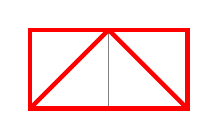
\begin{tikzpicture}
    \draw[gray] (0,0) grid (2,1);
    \draw[red,ultra thick] (0,0) rectangle (2,1);
    \draw[red,ultra thick] (0,0)--(1,1) (1,1)--(2,0) (2,0)--(0,0);
  \end{tikzpicture}
  ~
  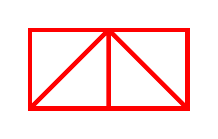
\begin{tikzpicture}
    \draw[gray] (0,0) grid (2,1);
    \draw[red,ultra thick] (0,0) rectangle (2,1);
    \draw[red,ultra thick] (0,0)--(1,1) (1,1)--(2,0) (2,0)--(0,0) (1,0)--(1,1);
  \end{tikzpicture}
  ~
  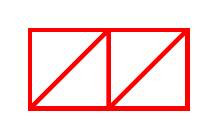
\begin{tikzpicture}
    \draw[gray] (0,0) grid (2,1);
    \draw[red,ultra thick] (0,0) rectangle (2,1);
    \draw[red,ultra thick] (0,0)--(1,1) (1,1)--(1,0) (1,0)--(2,1);
  \end{tikzpicture}
  ~
  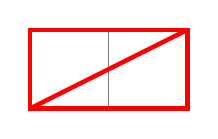
\begin{tikzpicture}
    \draw[gray] (0,0) grid (2,1);
    \draw[red,ultra thick] (0,0) rectangle (2,1);
    \draw[red,ultra thick] (0,0)--(2,1);
  \end{tikzpicture}
  ~
  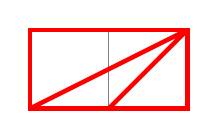
\begin{tikzpicture}
    \draw[gray] (0,0) grid (2,1);
    \draw[red,ultra thick] (0,0) rectangle (2,1);
    \draw[red,ultra thick] (0,0)--(2,1) (1,0)--(2,1);
  \end{tikzpicture}
  ~
  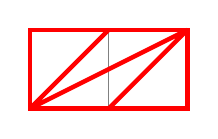
\begin{tikzpicture}
    \draw[gray] (0,0) grid (2,1);
    \draw[red,ultra thick] (0,0) rectangle (2,1);
    \draw[red,ultra thick] (0,0)--(2,1) (1,0)--(2,1) (0,0)--(1,1);
  \end{tikzpicture}
  \caption{
    All six partitions of the $2 \times 1$ grid into triangles with
    gridpoint vertices, up to dihedral action.
  }
\end{figure}

\begin{figure}[ht!]
  \centering
  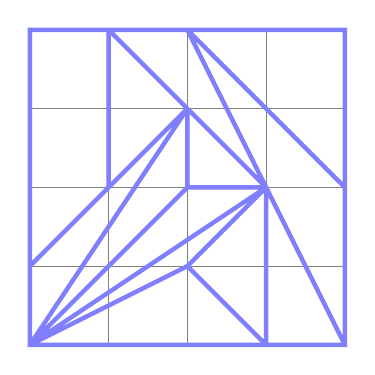
\begin{tikzpicture}
    \draw[gray] (0,0) grid (4,4);
    \draw[blue!50,ultra thick]
      (0,0) rectangle (4,4)
      (0,0)--(0,1)
      (0,0)--(2,1)
      (0,0)--(2,2)
      (0,0)--(2,3)
      (0,0)--(3,2)
      (0,1)--(2,3)
      (1,2)--(1,4)
      (1,4)--(2,3)
      (2,1)--(3,0)
      (2,1)--(3,2)
      (2,2)--(2,3)
      (2,2)--(3,2)
      (2,3)--(3,2)
      (2,4)--(4,2)
      (3,0)--(3,2)
      (4,0)--(2,4)
      ;
  \end{tikzpicture}
  \caption{
    An example of a partitions of the $4 \times 4$ grid into triangles with no
    ``empty'' gridpoints.
  }
\end{figure}
\begin{question}
  How many such partitions exist?
\end{question}

\begin{related}
  \item What if these are counted up to rotation/reflection?
  \item What if this is done on a triangular/hexagonal grid?
  \item How many partitions with the maximal number of triangles? With $k$ triangles?
  \item What if all triangles must be right triangles? Acute? Obtuse?
  \item What if each gridpoint must touch a triangle?
  What is the minimum number of faces?
  \item What if each gridpoint must touch as many triangles as possible?
  What is the minimum number of faces? What's the expected number of faces?
  (i.e. there's no way to draw a new edge?)
  \item What if this is done on a grid in hyperbolic space?
\end{related}

\begin{note}
  $a_1(n) = A051708(n)$
\end{note}

\begin{references}
  \item \url{https://oeis.org/A051708}
  \item \url{https://codegolf.stackexchange.com/q/176646/53884}
\end{references}

\end{document}
